\documentclass{article}

\usepackage[margin = 1in]{geometry}

\usepackage{amsmath, graphicx, makecell}
\graphicspath{ {./images/} }

\title{Ch. 14 Solutions}
\author{Principles of Microeconomics}
\date{\today}

\begin{document}

\maketitle

\section*{Quick Quiz}

\begin{enumerate}

\item (c) -- His explicit cost is \$100 for seeds. His implicit cost is \$200 from the income he forewent by not teaching banjo lessons.

\item (a) -- His explicit cost is \$10 for ingredients. His implicit cost is \$40 from the income he forewent by not mowing his neighbor's lawn. That means his accounting profit is $60 - 10 = 50$, and his economic profit is $60 - (10 + 40) = 10$. 

\item (a) -- She got two additional bushels from her second seed. Since the seeds have diminishing marginal productivity, she will get fewer than two additional bushels from her third seed. Therefore, she must get fewer than 7 bushels from 3 bags. 

\item (d) -- The production function gets flatter because each additional unit of input increases output by less than the last unit of input. The total cost curve gets steeper because each additional unit of output requires the firm to increase its inputs by more than the last unit of output did. 

\item (d) -- Increasing output by one costs \$8, so marginal cost is \$8. \$5,008 divided by 1,000 units is roughly \$5, so average total cost is \$5.

\item (c) -- Since marginal cost is less than average total cost, producing one more unit will pull average total cost down.

\item (b) -- The license fee is a fixed cost because it doesn't depend on how much output the firm produces. Fixed costs factor into the average total cost and the average fixed cost curves. 

\item (a) -- Specialization makes workers more productive, so the firm's marginal product of labor increases. If the marginal product of labor increases, that means the firm's marginal cost will fall which will in turn drag down average total cost. If average total cost falls, the firm is exhibiting economies of scale.

\item (d) -- As production increases, average total cost increases. That means Boeing exhibits diseconomies of scale. 

\end{enumerate}

\section*{Questions for Review}

\begin{enumerate}

\item Profit = Total Revenue - Total Cost

\item The money that firms spend establishing their business could earn interest if the firm saved it instead. We call the interest that they would have earned the cost of capital. Since the cost of capital in this case is an implicit cost -- it doesn't require a cash outlay -- accountants would ignore it.

\item The marginal product of an input is the change in output from a one unit increase in that input. Diminishing marginal product is the idea that each additional unit of an input increases output by less than the last unit of that input did.

\item The production function is increasing at a decreasing rate because each additional unit of labor increases output by less than the last unit of labor did.

	\begin{center}
	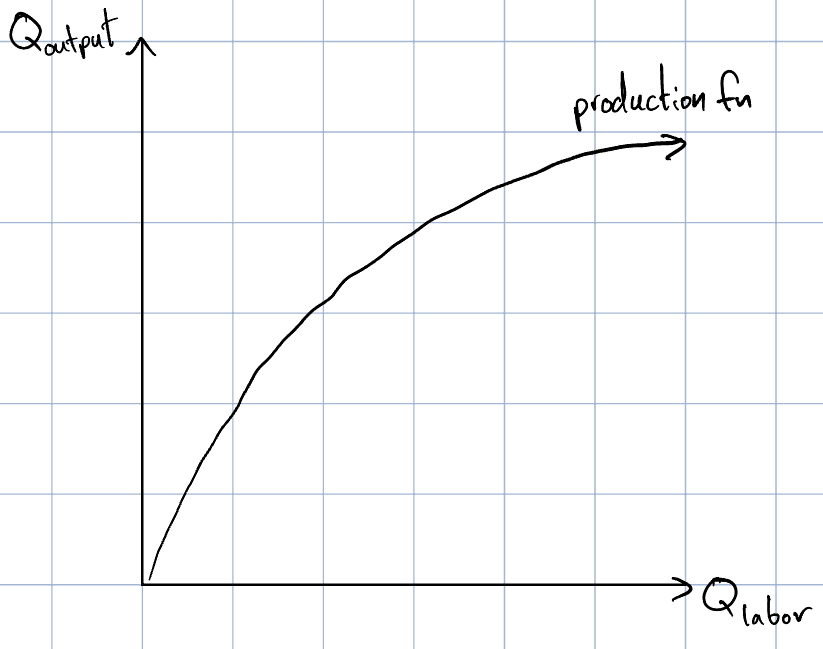
\includegraphics[width = 0.3\textwidth]{ch14_qfr4_production}
	\end{center}
	
	The total cost curve is increasing at an increasing rate because each additional unit of output requires hiring more additional labor than the last unit did. That makes each additional unit of output more expensive to produce than the last.
	
	\begin{center}
	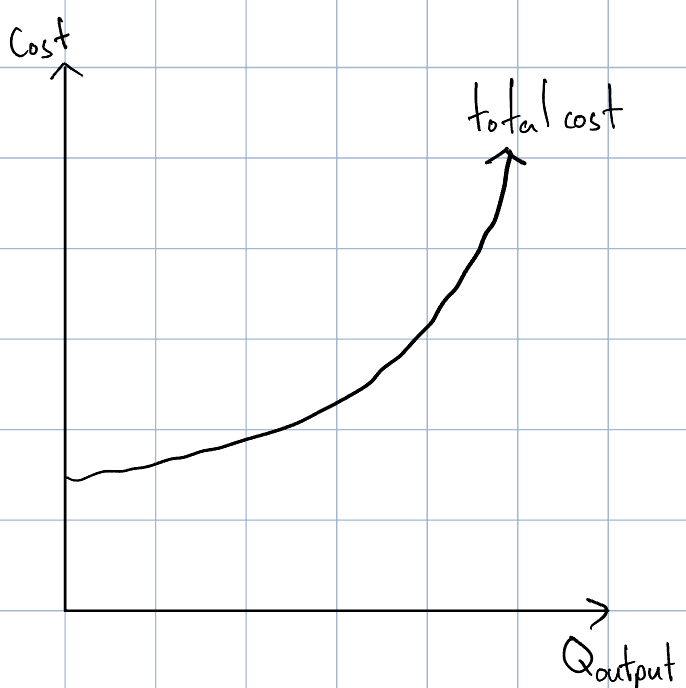
\includegraphics[width = 0.3\textwidth]{ch14_qfr4_totalcost} 
	\end{center}
	
\item Total cost is how much the firm has to spend on inputs to produce all of its output. Mathematically, it's the sum of the firm's explicit and implicit costs. Alternatively, it's the sum of the firm's fixed and variable costs.

Average total cost is the cost of producing a typical unit of output. Mathematically, it's total cost divided by total output.

Marginal cost is the cost of producing an additional unit of output. Mathematically, it's the change in total cost divided by the change in total output.

\item \phantom{x}

	\begin{center}
	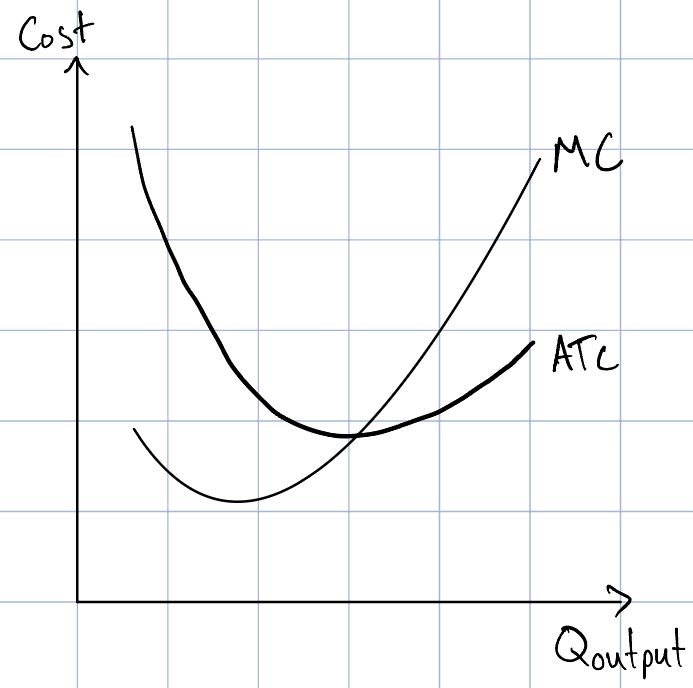
\includegraphics[width = 0.3\textwidth]{ch14_qfr6}
	\end{center}

As output increases, marginal cost typically decreases at first before eventually increasing. That's because the marginal product of labor typically increases at first which drives down marginal cost, but then eventually it decreases which drives up marginal cost.

Average total cost has a similar U-shape. It decreases at first because average total cost equals the sum of average fixed cost and average variable cost, and average fixed cost falls rapidly at fist as the fixed costs are spread across the first few units of output. Eventually, average total cost increases because diminishing marginal product causes average variable costs to increase, and the increase in average variable cost overwhelms the decrease in average fixed cost. 

The marginal cost curve intersects the average total cost curve at its minimum. If marginal cost is below average total cost, then producing an additional unit of output will pull the average total cost curve down. If marginal cost is above average total cost, then producing an additional unit of output will pull the average total cost curve up. In other words, if marginal cost is below average total cost, average total cost is decreasing, and if marginal cost is above average total cost, then average total cost is increasing. That means the average total cost curve flips from decreasing to increasing when the marginal cost curve moves from below it to above it. Therefore, the marginal cost curve intersects average total cost curve at its minimum.

\item In the long run, firms' ATC curves are a flatter U-shape and lie below its short run ATC curves. That's because in the long run there are no fixed costs -- all costs are variable. As a result, firms have more flexibility to choose their inputs and keep their costs low.

\item A company exhibits economies of scale if its average total costs decline as its output increases. Economies of scale often occur when employing more labor allows for greater specialization and therefore greater productivity. 

A company exhibits diseconomies of scale if its average total costs increase as its output increases. Diseconomies of scale often occur when companies get so large that there are coordination problems that make it less productive.  

\end{enumerate}

\section*{Problems and Applications}

\begin{enumerate}

\item

	\begin{enumerate}
	
	\item opportunity cost
	
	\item average total cost
	
	\item fixed cost
	
	\item variable cost
	
	\item total cost
	
	\item marginal cost
	
	\end{enumerate}
	
\item 

	\begin{enumerate}
	
	\item The opportunity cost of a choice is what you give up to make it.
	
	\item $\$350,000 + \$80,000 = \$430,000$
	
	\item $\$400,000 - \$350,000 = \$50,000$
	
	\item She should not. Her economic profit is negative because her opportunity cost is greater than her total revenue. In other words, she would be better off if she remained a vampire hunter. 
	
	\item It would need to generate more than her opportunity cost, \$430,000. 
	
	\end{enumerate}
	
\item

	\begin{enumerate}
	
	\item \phantom{x}
	
		\begin{center}
		\begin{tabular}{ c | c | c}
		\textbf{Hours} & \makecell{\textbf{Quantity of Fish}\\\textbf{(in pounds)}} & \makecell{\textbf{Marginal}\\ \textbf{Product}} \\
		\hline
		0 & 0 & -- \\
		1 & 10 & 10 \\
		2 & 18 & 8 \\
		3 & 24 & 6 \\
		4 & 28 & 4 \\
		5 & 30 & 2 \\
		\end{tabular}
		\end{center}
		
	\item The production function is increasing at a decreasing rate because the fisherman's marginal product of time is diminishing. The more hours he works, the less productive each additional hour is.
	
		\begin{center}
		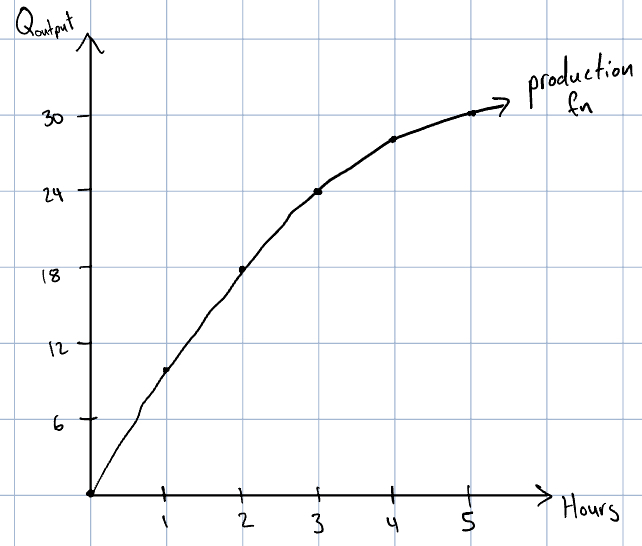
\includegraphics[width = 0.3\textwidth]{ch14_paa3b}
		\end{center}
		
	\item The total cost curve is increasing at an increasing rate. Because the fisherman's marginal product of time is diminishing, each additional fish that he catches takes him more time to catch than the last one. That means his opportunity cost accelerates as he catches more fish.
	
		\begin{center}
		\begin{tabular}{ c | c | c | c | c }
		\textbf{Hours} & \makecell{\textbf{Quantity of Fish}\\\textbf{(in pounds)}} & \makecell{\textbf{Fixed}\\\textbf{{Cost}}} & \makecell{\textbf{Variable}\\\textbf{Cost}} & \makecell{\textbf{Total}\\\textbf{Cost}} \\
		\hline
		0 & 0 & 10 & 0 & 10 \\
		1 & 10 & 10 & 5 & 15 \\
		2 & 18 & 10 & 10 & 20  \\
		3 & 24 & 10 & 15 & 25 \\
		4 & 28 & 10 & 20 & 30 \\
		5 & 30 & 10 & 25 & 35 \\
		\end{tabular}
		
		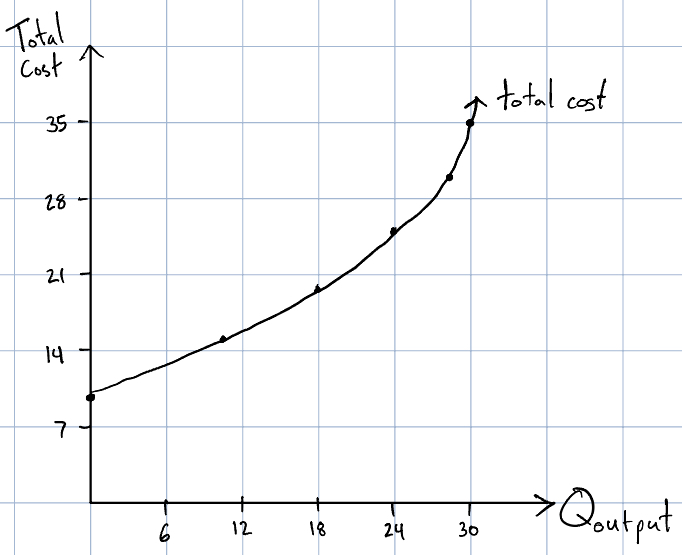
\includegraphics[width = 0.3\textwidth]{ch14_paa3c}
		\end{center}
	
	\end{enumerate}
	
\item \phantom{x}

	\begin{center}
	\begin{tabular}{| c | c | c | c | c | c |}
	\hline
	Workers & Output & \makecell{Marginal\\Product} & \makecell{Total\\Cost} & \makecell{Average\\Total\\Cost} & \makecell{Marginal\\Cost} \\
	\hline
	0 & 0 & -- & 200 & -- & -- \\
	\hline
	1 & 20 & 20 & 300 & 15 & 5 \\
	\hline
	2 & 50 & 30 & 400 & 8 & 3.33 \\
	\hline
	3 & 90 & 40 & 500 & 5.56 & 2.5 \\
	\hline
	4 & 120 & 30 & 600 & 5 & 3.33 \\
	\hline
	5 & 140 & 20 & 700 & 5 & 5 \\
	\hline
	6 & 150 & 10 & 800 & 5.33 & 10 \\
	\hline
	7 & 155 & 5 & 900 & 5.81 & 20 \\
	\hline
	\end{tabular}
	\end{center}
	
	\begin{enumerate}
	
	\item At first, marginal product is increasing. Then, it diminishes. Additional workers might be increasingly productive at first because having multiple workers allows each worker to specialize and become better at their particular task. Eventually, additional workers might become decreasingly productive because there isn't enough work for each worker to operate at maximum capacity or because it gets harder to coordinate a larger work force. 
	
	\item See above.
	
	\item Average total cost decreases at first and increases later.
	
	\item Marginal cost decreases at first and increases later.
	
	\item Marginal product increases at first and decreases later. Marginal cost decreases at first and increases later. The trend in marginal product explains the trend in marginal cost. Since workers get increasingly productive at first, it requires less additional labor to produce an additional unit of output. Less additional labor means lower marginal costs. When workers get less productive, it requires more additional labor to produce an additional unit of output. Hiring more additional labor means higher marginal costs.
	
	\item When marginal cost is lower than average total cost, average total cost is decreasing because producing additional units at lower than average cost pulls the average down. When marginal cost is higher than average total cost, average total cost is increasing because producing additional units at higher than average cost pulls the average up. Marginal cost intersects average total cost at average total cost's minimum because that's where average total cost switches from decreasing to increasing.
	
	\end{enumerate}
	
\item No, I shouldn't. At 600 consoles, total cost is $600 * \$300 = \$180,000$. At 601 consoles, total cost is $601 * \$301 = \$180,901$. That means the marginal cost of producing the 601st console is \$901. Therefore, producing another console would cost me more than the person is offering. 

\item

	\begin{enumerate}
	
	\item Its fixed cost is \$300.
	
	\item The change in total cost equals the change in variable cost. That's because fixed cost doesn't change when the quantity of output changes, so the change in total cost is entirely the change in variable cost. Mathematically,
	
	\begin{align*}
	\Delta TC &= TC_2 - TC_1 \\
	&= (FC + VC_2) - (FC + VC_1) \\
	&= FC + VC_2 - FC - VC_1 \\
	&= VC_2 - VC_1 \\
	&= \Delta VC
	\end{align*}
	
	\begin{center}
	\begin{tabular}{c | c | c | c | c}
	Quantity & TC & VC & $MC = \Delta TC$ & $MC = \Delta VC$ \\
	\hline
	0 dozen pizzas & \$300 & \$0 & -- & -- \\
	1 & 350 & 50  & 50 & 50 \\
	2 & 390 & 90 & 40 & 40 \\
	3 & 420 & 120 & 30 & 30 \\
	4 & 450 & 150 & 30 & 30 \\
	5 & 490 & 190 & 40 & 40 \\
	6 & 540 & 240 & 50 & 50 \\
	\end{tabular}
	\end{center}
	
	\end{enumerate}
	
\item The efficient scale of the company is 4 houses painted per month. 

	\begin{center}
	\begin{tabular}{| c | c | c | c | c | c | c | c |}
	\hline
	\makecell{Quantity of\\Houses\\Painted per\\Month} & 1 & 2 & 3 & 4 & 5 & 6 & 7 \\
	\hline
	\makecell{Variable\\Costs} & \$10 & \$20 & \$40 & \$80 & \$160 & \$320 & \$640 \\
	\hline
	$AFC = \frac{FC}{Q}$ & 200 & 100 & 66.67 & 50 & 40 & 33.33 & 28.57 \\
	\hline
	$AVC = \frac{VC}{Q}$ & 10 & 10 & 13.33 & 20 & 32 & 53.33 & 91.43 \\
	\hline
	$ATC$ & 210 & 110 & 80 & 70 & 72 & 86.67 & 120 \\
	\hline
	\end{tabular}
	\end{center}
	
\item

	\begin{enumerate}
	
	\item A lump-sum tax is a single payment that every person or firm has to pay regardless of their circumstances. Since it doesn't depend on the quantity of output produced, it's a fixed cost. Therefore, the average fixed cost and average total cost curves shift. Marginal cost doesn't shift because marginal cost just depends on variable cost (as we saw in 4).

		\begin{center}
		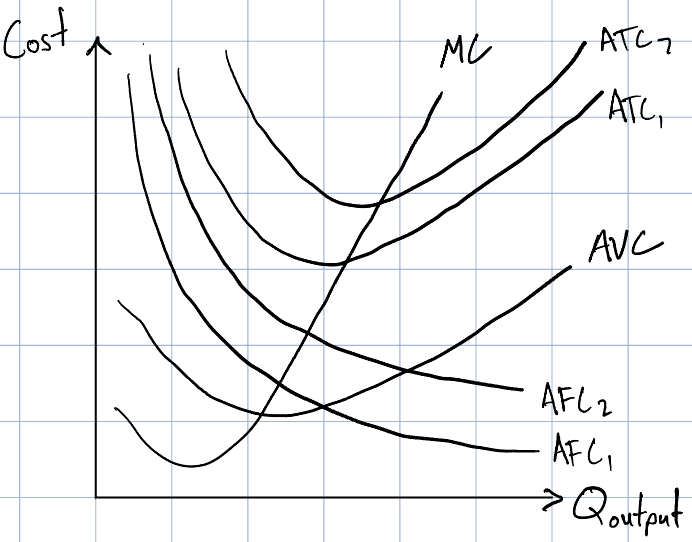
\includegraphics[width = 0.3\textwidth]{ch14_paa8a}
		\end{center}
	
	\item The per-burger tax is a variable cost, so the average variable cost, average total cost, and marginal cost curves shift.
	
		\begin{center}
		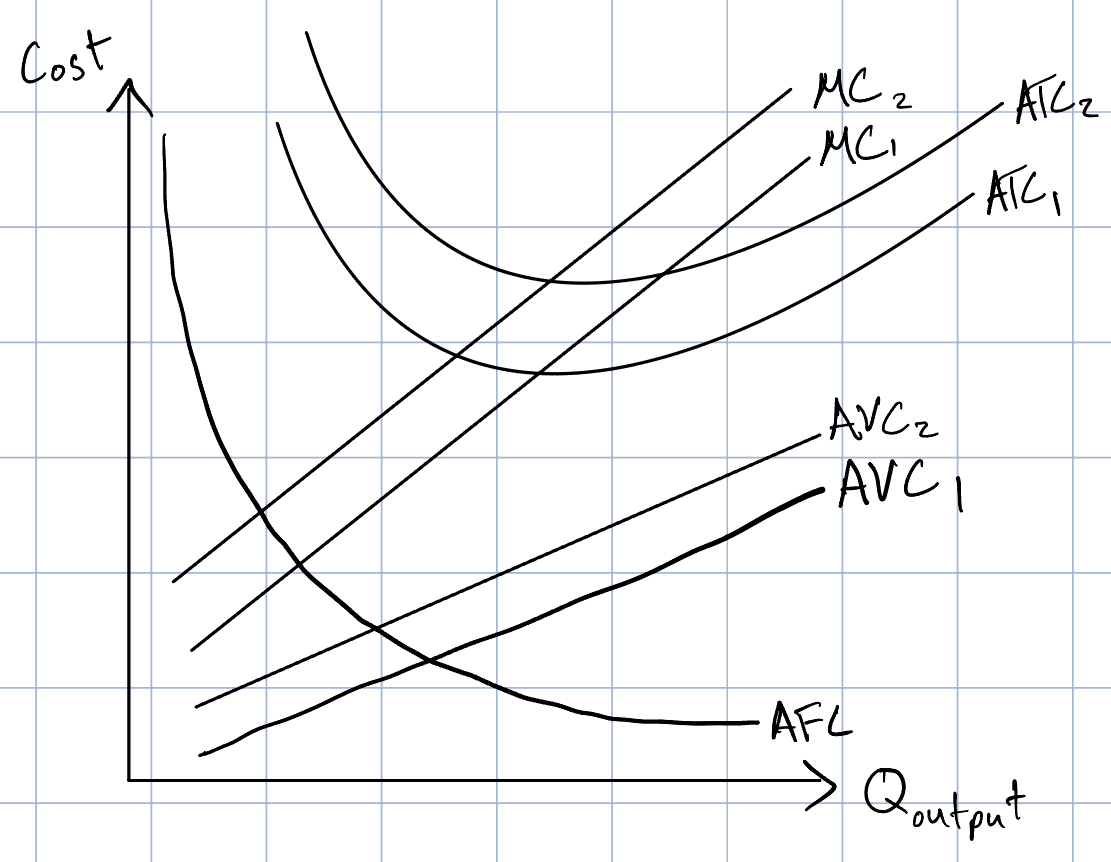
\includegraphics[width = 0.3\textwidth]{ch14_paa8b}
		\end{center}
	
	\end{enumerate}
	
\item 
	\begin{enumerate}
	
	\item \phantom{x}
	
		\begin{center}
		\begin{tabular}{c | c | c | c | c | c}
		Quantity & VC & TC & AVC & ATC & MC\\
		\hline
		0 & 0 & 30 & -- & -- & -- \\
		1 & 10 & 40 & 10 & 40 & 10 \\
		2 & 25 & 55 & 12.5 & 27.5 & 15 \\
		3 & 45 & 75 & 15 & 25 & 20 \\
		4 & 70 & 100 & 17.5 & 25 & 25 \\
		5 & 100 & 130 & 20 & 26 & 30 \\
		6 & 135 & 165 & 22.5 & 27.5 & 35
		\end{tabular}
		\end{center}
		
	\item When MC is less than ATC, producing one more unit pulls ATC down, so ATC is decreasing. Similarly, when MC is greater than ATC, producing one more unit pulls ATC up, so ATC is increasing. Therefore, when MC intersects ATC, ATC switches from decreasing to increasing, so ATC is at a minimum.
	
	When MC is greater than AVC, producing one more unit pulls AVC up, so AVC is increasing. It intersects with AVC when quantity is one because at that quantity marginal cost equals variable cost, and the denominator of average variable cost is one.
		\begin{center}
		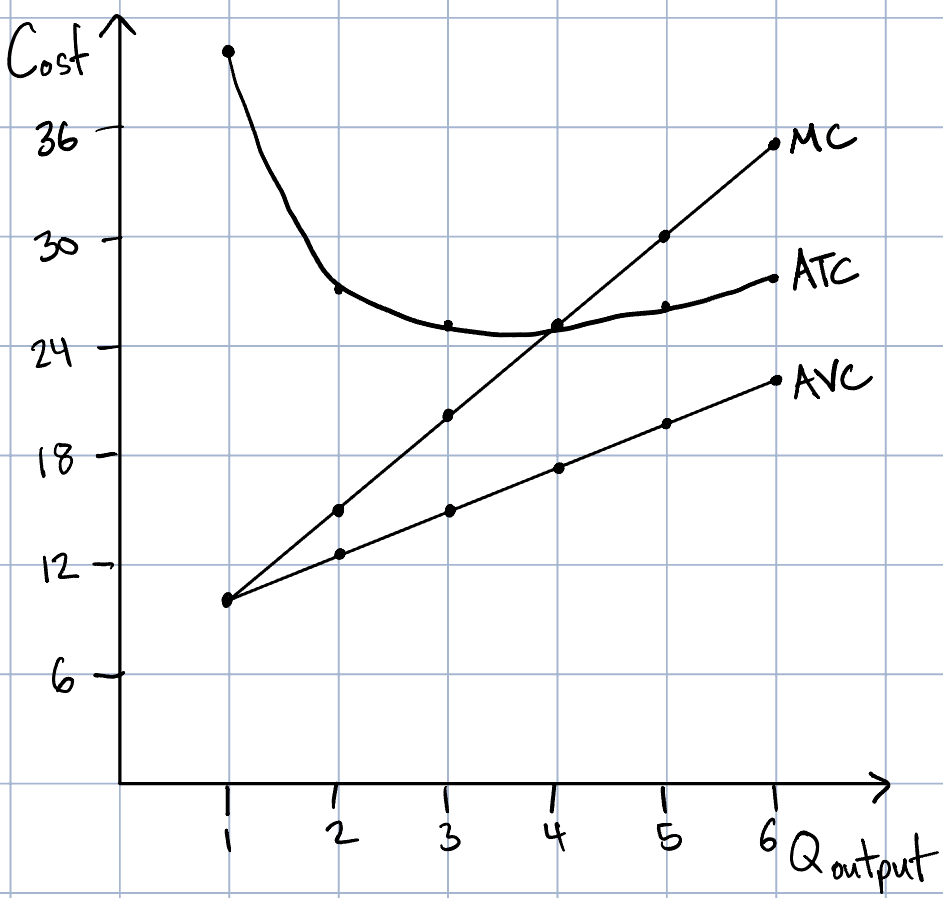
\includegraphics[width = 0.3\textwidth]{ch14_paa9b}
		\end{center}
	
	\end{enumerate}
	
\item Below is a table of each firm's ATC.

	\begin{center}
	\begin{tabular}{| c | c | c | c | c | c | c | c |}
	\hline
	\textbf{Quantity} & 1 & 2 & 3 & 4 & 5 & 6 & 7 \\
	\hline
	\textbf{Firm A} & \$60 & \$35 & \$26.67 & \$22.5 & \$20 & \$18.33 & \$17.14 \\
	\hline
	\textbf{Firm B} & 11 & 12 & 13 & 14 & 15 & 16 & 17 \\
	\hline
	\textbf{Firm C} & 21 & 17 & 16.33 & 16.5 & 17 & 17.67 & 18.43 \\
	\hline
	\end{tabular}
	\end{center}
	
	Firm A experiences economies of scale because their ATC decreases as their output increases. Firm B experiences diseconomies of scale because their ATC increases as their output increases. Firm C experiences economies of scale for low levels of output and diseconomies of scale for high levels of output.

\end{enumerate}

\end{document}